\subsection{Planejamento do Experimento Controlado}
\label{subsec:plan_exp}

Após a fase de ideação, iniciou-se o planejamento do experimento. Este estudo busca responder à primeira questão específica de pesquisa do estudo de caso, conforme descrito na Subseção \ref{subsec:estudo-questao}. O experimento consiste na comparação entre duas versões do produto, avaliando aspectos relacionados à qualidade em uso.

A literatura evidencia a complexidade na definição de métricas que representem com precisão a entrega de valor almejada \cite{crook_seven_2009, larsen_statistical_2024}. Para mitigar as limitações inerentes a uma única métrica, optou-se por adotar múltiplas medidas que refletem alguns dos objetivos estratégicos do negócio, utilizando normas de referência para assegurar maior confiabilidade e reprodutibilidade dos resultados.

No contexto da Engenharia de \textit{Software}, as métricas podem ser classificadas segundo diferentes critérios. Quanto à \textbf{forma de coleta}, uma métrica pode ser \textbf{direta}, quando obtida sem necessidade de cálculos ou transformações, ou \textbf{indireta}, quando derivada a partir de outras métricas. Além disso, as métricas podem ser \textbf{objetivas}, caso sua mensuração seja independente da interpretação do avaliador, ou \textbf{subjetivas}, quando dependem da percepção do avaliador ou do próprio usuário \cite{wohlin_experimentation_2012}.

Outro fator relevante é o tipo de \textbf{escala} utilizada, que influencia as análises estatísticas aplicáveis. As escalas \textbf{nominais} classificam os dados sem uma ordem definida, enquanto as escalas \textbf{ordinais} estabelecem uma hierarquia, mas sem diferenças proporcionais entre os valores. Já as escalas \textbf{intervalares} permitem quantificar diferenças, embora sem um zero absoluto, ao passo que as escalas \textbf{de razão} possuem um zero absoluto e possibilitam comparações proporcionais \cite{wohlin_experimentation_2012}.

Dessa forma, na seleção das métricas para este experimento, tomou-se como base a norma \citeonline{nbr9241}, considerando o contexto do filtro de nível de dificuldade e da criação de atividades, funcionalidades diretamente relacionadas à hipótese analisada. Assim, as métricas adotadas foram definidas para capturar diferentes dimensões da qualidade em uso, sendo elas:

\begin{itemize}
  \item \textbf{Número de utilizações do filtro de nível de dificuldade}: métrica objetiva e direta, mensurada na escala de razão. Representa um indicador quantitativo da subcaracterística de \textit{utilidade}, relacionada à satisfação do usuário.
  \item \textbf{Número de atividades criadas}: métrica objetiva e direta, também mensurada na escala de razão. Relaciona-se à eficácia do produto, indicando se a plataforma auxilia o usuário a atingir seus objetivos.
  \item \textbf{Número de exercícios selecionados}: métrica objetiva e direta, mensurada na escala de razão. Assim como a métrica anterior, reflete a eficácia do produto, avaliando o engajamento dos usuários na realização de atividades propostas.
\end{itemize}

A escolha dessas métricas visa garantir que os dados coletados possibilitem uma análise estatística confiável e alinhada aos objetivos do estudo. Ademais, a utilização de múltiplas métricas reduz o risco de interpretações enviesadas e amplia a compreensão dos impactos das modificações no produto. A relação dessas métricas com as características e subcaracterísticas da qualidade em uso é apresentada na Tabela \ref{tab:metricas_qualidade_uso}.

\begin{table}[h]
    \centering
    \renewcommand{\arraystretch}{1.2}
    \setlength{\tabcolsep}{3pt}
    \begin{tabular}{|p{3cm}|p{3.5cm}|p{3.75cm}|p{4.75cm}|}
        \hline
        \textbf{Característica} & \textbf{Subcaracterística} & \textbf{Métrica} & \textbf{Descrição} \\
        \hline
        \multirow{1}{*}{Satisfação} & Utilidade & Número de utilizações do filtro de nível de dificuldade & Mede a utilidade da funcionalidade ao quantificar a frequência de uso dentro do período observado. \\
        \hline
        \multirow{2}{*}{Eficácia} & Eficácia & Número de atividades criadas & Avalia a eficácia do produto em auxiliar o usuário a alcançar seus objetivos, especificamente na criação de listas de exercícios. \\
        \cline{2-4}
        & Eficácia & Número de exercícios selecionados & Mede a eficácia do produto na seleção de exercícios para atividades, refletindo o engajamento do usuário. \\
        \hline
    \end{tabular}
    \caption{Métricas Escolhidas de Qualidade em Uso}
    \label{tab:metricas_qualidade_uso}
\end{table}

Além disso, para incluir a percepção dos profissionais envolvidos na ponderação dos resultados, o peso de cada métrica foi determinado pelo método AHP, conforme proposto pelo modelo QATCH, convertendo avaliações qualitativas em pesos quantitativos (ver Subseções \ref{subsec:qatch} e \ref{subsec:ahp}). Para isso, foi realizada uma reunião para definir a importância relativa de cada métrica e característica em diferentes níveis de agregação. Essa avaliação foi feita por pares, considerando a relação entre satisfação e eficácia (no nível de característica, para calcular a qualidade em uso) e entre o número de listas criadas e exercícios selecionados (no nível de métrica, para calcular a eficácia). Essa relação é ilustrada na Figura \ref{fig:qatch_experiment}.

\begin{figure}
    \centering
    \caption{Modelo de Agregação QATCH do Experimento}
    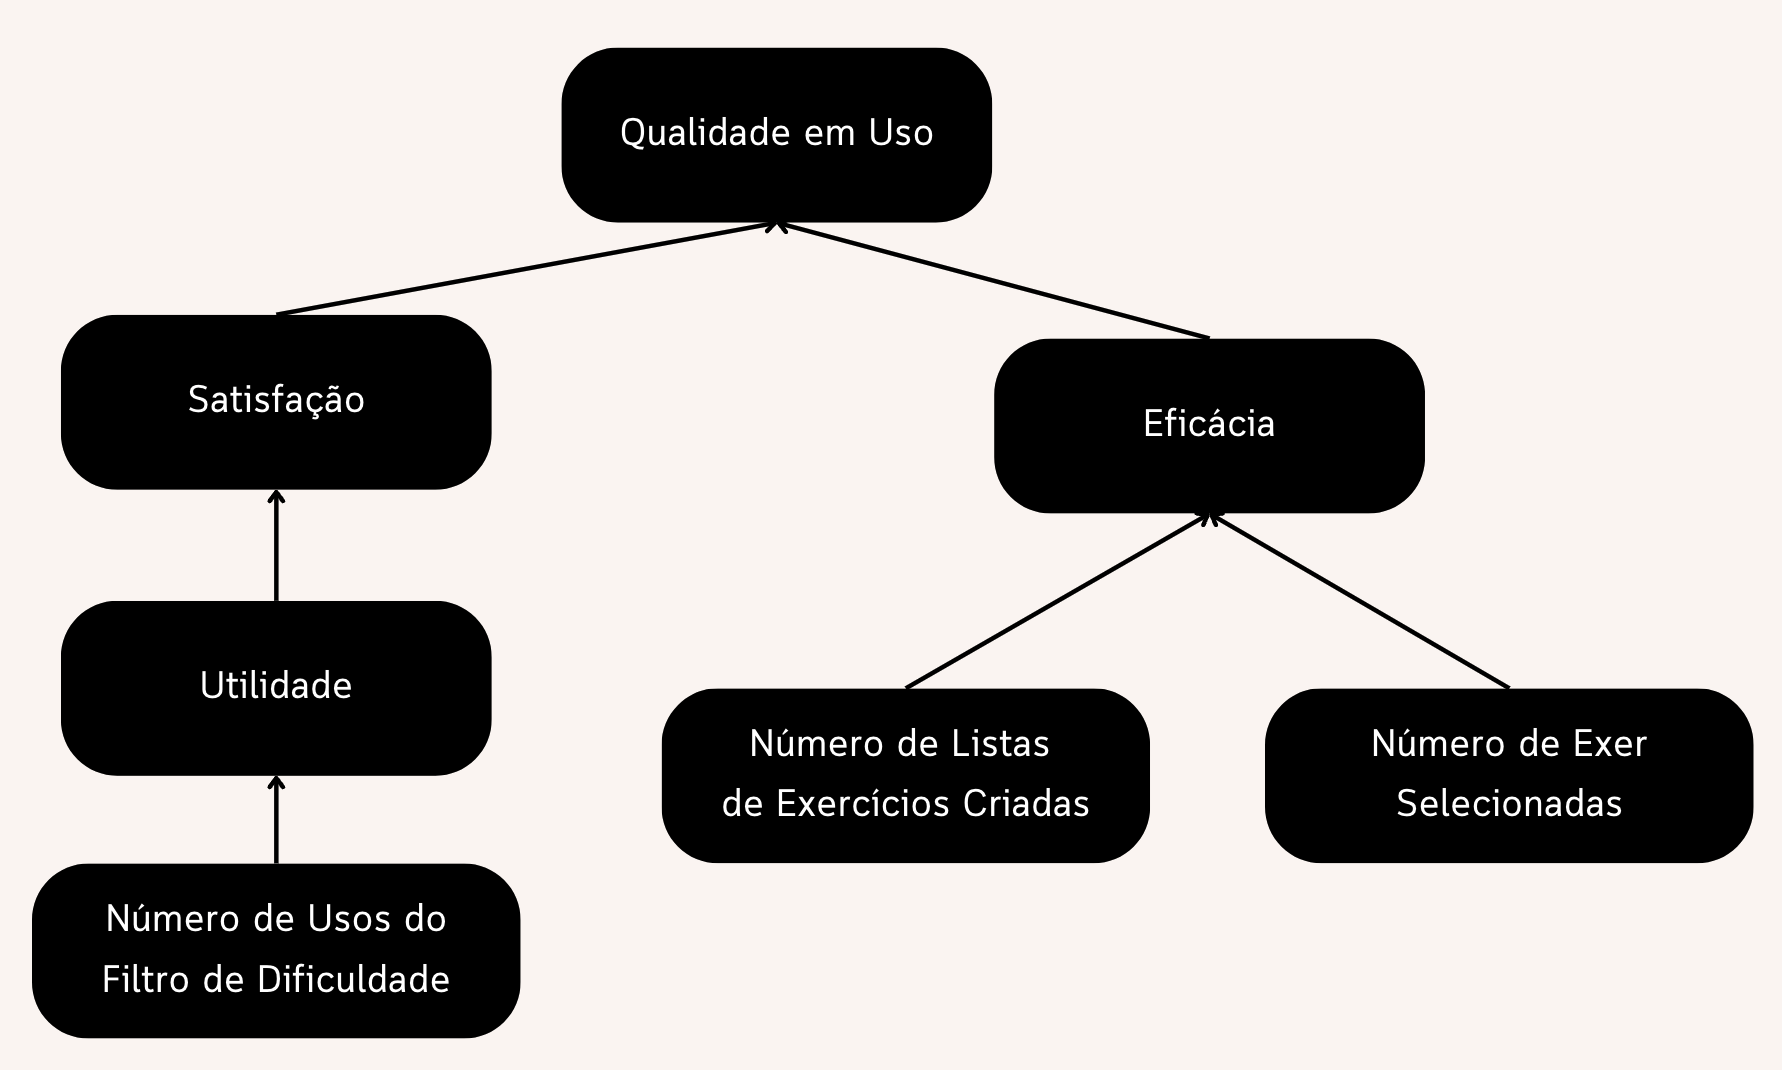
\includegraphics[width=1\linewidth]{figuras/qach_experiment.png}
    \begin{center}
        \text{Fonte: Autor}
    \end{center}
    \label{fig:qatch_experiment}
\end{figure}

Após discussões, os pesos relativos foram definidos em consenso, sendo os resultados apresentados nas Tabelas \ref{tab:ahp-metrics} e \ref{tab:ahp-characteristics}. Com esses valores estabelecidos, foi possível calcular os pesos quantitativos. A métrica de número de listas de exercícios criadas possui peso de 0.8889, enquanto a métrica de número de exercícios selecionados tem peso de 0.111. Juntas, representam a característica de eficácia. Para as características, os pesos são 0.8333 para satisfação e 0.1667 para eficácia. A soma desses valores gera um indicador único de qualidade em uso para cada usuário (este cálculo é detalhado na Subseção \ref{subsec:qatch}). Essa relação é apresentada visualmente na Figura \ref{fig:qatch_pesos}.

\begin{table}[ht]
    \centering
    \caption{Importância Relativa das Métricas de Eficácia}
    \begin{tabular}{|p{4cm}|p{4cm}|p{6.5cm}|}
        \hline
        Métrica & Nº de Listas Criadas & Nº de Exercícios Selecionados \\ \hline
        Nº de Listas Criadas & - & Muito Mais Importante \\ \hline
        Nº de Exercícios Selecionados & - & - \\ \hline
    \end{tabular}
    \begin{center}
        \text{Fonte: Autor}
    \end{center}
    \label{tab:ahp-metrics}
\end{table}

\begin{table}[ht]
    \centering
    \caption{Importância Relativa das Características de Qualidade em Uso}
    \begin{tabular}{|p{4cm}|p{4cm}|p{6.5cm}|}
        \hline
        Característica & Satisfação & Eficácia \\ \hline
        Satisfação & - & Moderadamente Mais Importante \\ \hline
        Eficácia & - & - \\ \hline
    \end{tabular}
    \begin{center}
        \text{Fonte: Autor}
    \end{center}
    \label{tab:ahp-characteristics}
\end{table}

\begin{figure}
    \centering
    \caption{Pesos da Ponderação Agregada QATCH no Experimento}
    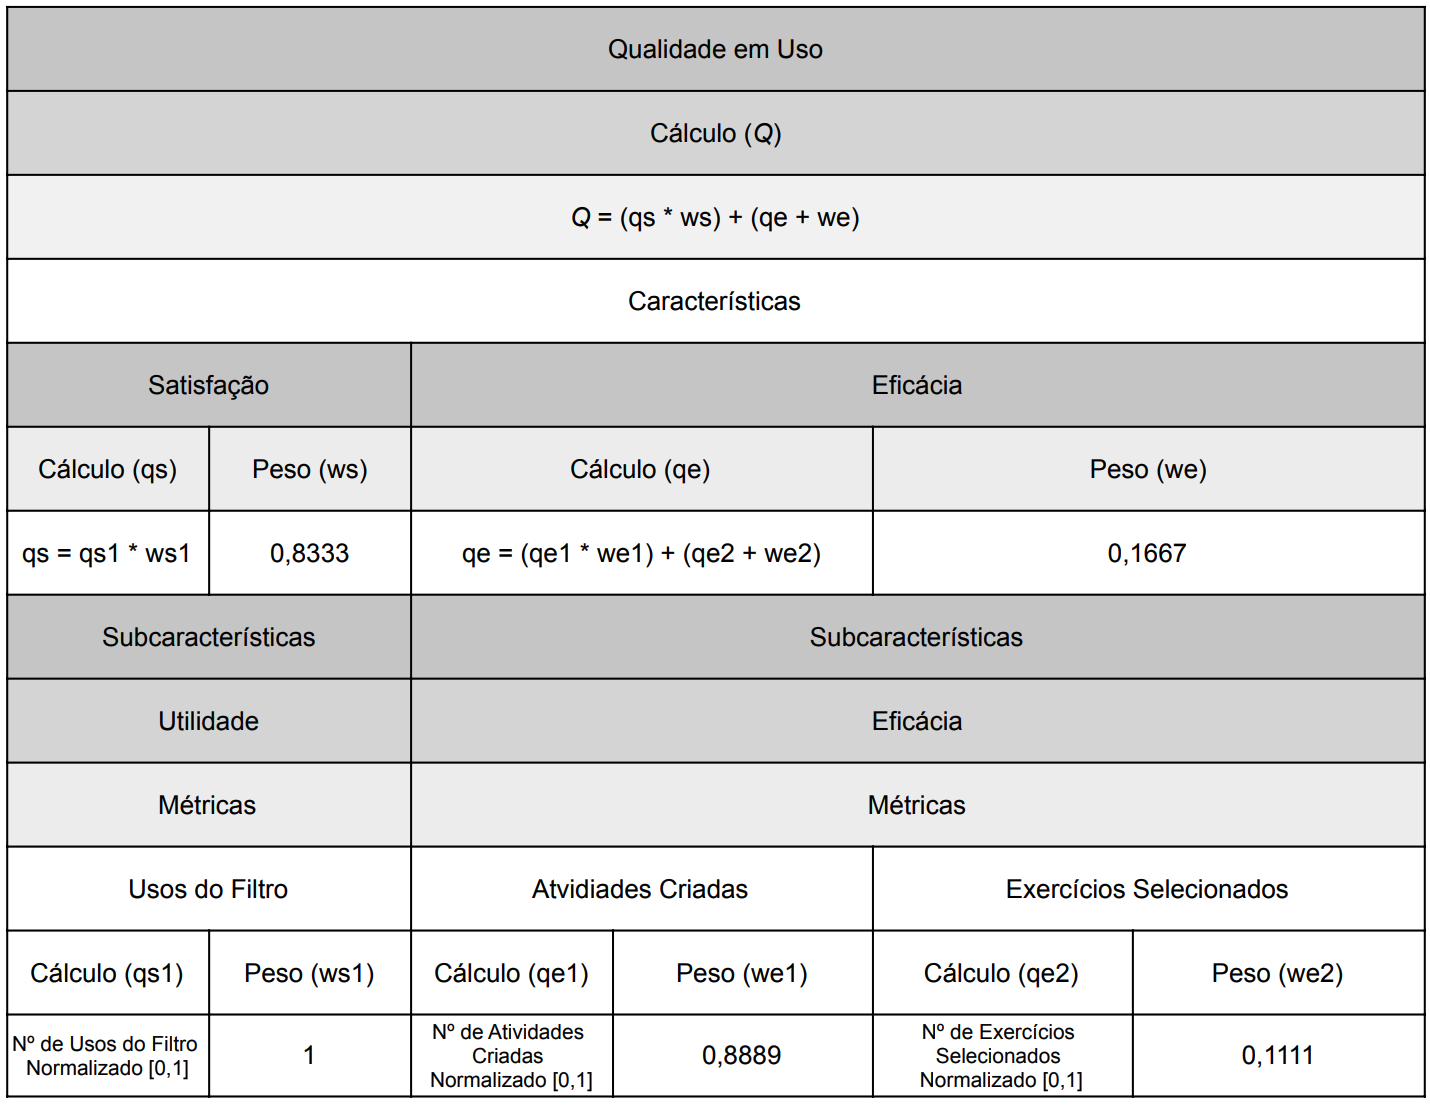
\includegraphics[width=1\linewidth]{figuras/tabela_exemplo_agregacao.png}
    \begin{center}
        \text{Fonte: Autor}
    \end{center}
    \label{fig:qatch_pesos}
\end{figure}


Desta forma então, os indicadores de qualidade em uso de cada usuário serão utilizados para se testar a hipótese formulada neste experimento, que servirá para responder a primeira questão específica deste estudo de caso, aprensentada na Subseção \ref{subsec:estudo-questao} (\textit{Durante o experimento, foi possível identificar diferença de qualidade em uso entre as versões de controle (A) e de tratamento (B) do produto, a partir de seu uso?}). Temos então as seguintes definições do experimento:


\begin{enumerate}
    \item \textbf{Escopo:} Analisar as versões A e B do produto com o propósito de avaliar sua efetividade e usabilidade das funcionalidads de filtragem de exercícios e criação de atividades, do ponto de vista do usuário final, no contexto do ambiente real de uso do sistema;
    
    \item \textbf{Objeto:} Versões de tratamento (A) e de controle (B) do produto sendo estudado;
    
    \item \textbf{Sujeitos:} Os participantes serão apenas os usuários docentes, já que são estes que criam listas de exercícios na plataforma. 
    
    \item \textbf{Populações:} Os sujeitos serão divididos em dois grupos: o de tratamento, composto pelos usuários beta, e o de controle, formado pelos demais usuários da base; Hoje os usuários beta representam cerca de 10\% da base total de usuários, uma maior discussão sobre esta divisão foi apresentada na Subseção \ref{subsubsec:variants};

    \item \textbf{Amostra:} a amostra coletada irá se referir a todos os docentes que criaram atividades no período e usaram algum dos filtros disponíveis; Não é possível estimar a proporção do tamanho da amostra dado que o mesmo dependerá do nível de atividade dos usuários durante o período;

    \item \textbf{Fator:} O fator analisado será a posição do filtro de nível de dificuldade no banco de questões. Dois tratamentos serão aplicados: um em que o filtro permanece na última posição (grupo de controle) e outro em que o filtro aparece em posição superior na listagem (grupo de tratamento);
    
    \item \textbf{Variáveis Independentes:} A posição do filtro será mantida de forma persistente para cada grupo, garantindo que cada usuário visualize sempre o filtro na mesma posição; A versão de controle será a mesma que já existe hoje, onde ele é o último da lista, como já abordado na Subseção \ref{subsec:plan_exp} e apresentado na Figura \ref{fig:selecao-questoes-controle}, já a versão de tratamento é apresentada na Figura \ref{fig:selecao-questoes-tratamento}, onde o filtro se torna o quarto da lista (esta posição foi ecolhida por que as três primeiras categorias são importantes para determinados fluxos de uso da aplicação, fazendo com que a equipe preferisse não alterá-los de lugar);
    
    \item \textbf{Variáveis Dependentes:} Número de vezes que cada docente utilizou o filtro, número de listas de exercícios criadas e número de exercícios selecionados. Essas variáveis serão normalizadas, ponderadas e agregadas para compor o indicador quantitativo \textit{Q}, conforme definido no modelo QATCH e apresentado anteriormente. Esse indicador busca expressar a percepção da qualidade em uso, observada em uma determinada versão do produto;

    \item \textbf{\textit{Design}:} Desta forma então, o experimento se tratará de um experimento de um fator e dois tratamentos, ou seja, haverão dois grupos onde cada um receberá um tratamento para o fator analisado, conforme apresentado na Tabela \ref{tab:design}; 
    
    \item \textbf{Hipóteses:} A hipótese nula a ser refutada neste experimento então será referente à qualidade em uso das duas versões analisadas, utilizando das métricas apresentadas anteriormente para analisar o contexto da funcionalidade avaliada, esta provém da suposição selecionada para teste que se refere à utilização do filtro de nível de dificuldade. Sendo assim temos as seguintes hipóteses:
    
    \begin{itemize}
        \item $H_0$: Não há diferença na percepção da qualidade em uso entre a versão de controle e a de tratamento ($Q_a = Q_b$);
        \item $H_1$: A percepção da qualidade em uso é maior na versão de controle em comparação à versão de tratamento ($Q_a > Q_b$);
        \item $H_2$: A percepção da qualidade em uso é menor na versão de controle em comparação à versão de tratamento ($Q_a < Q_b$).
    \end{itemize}
\end{enumerate}


\begin{figure}
    \centering
    \caption{Versão de Tratamento do Produto Analisado}
    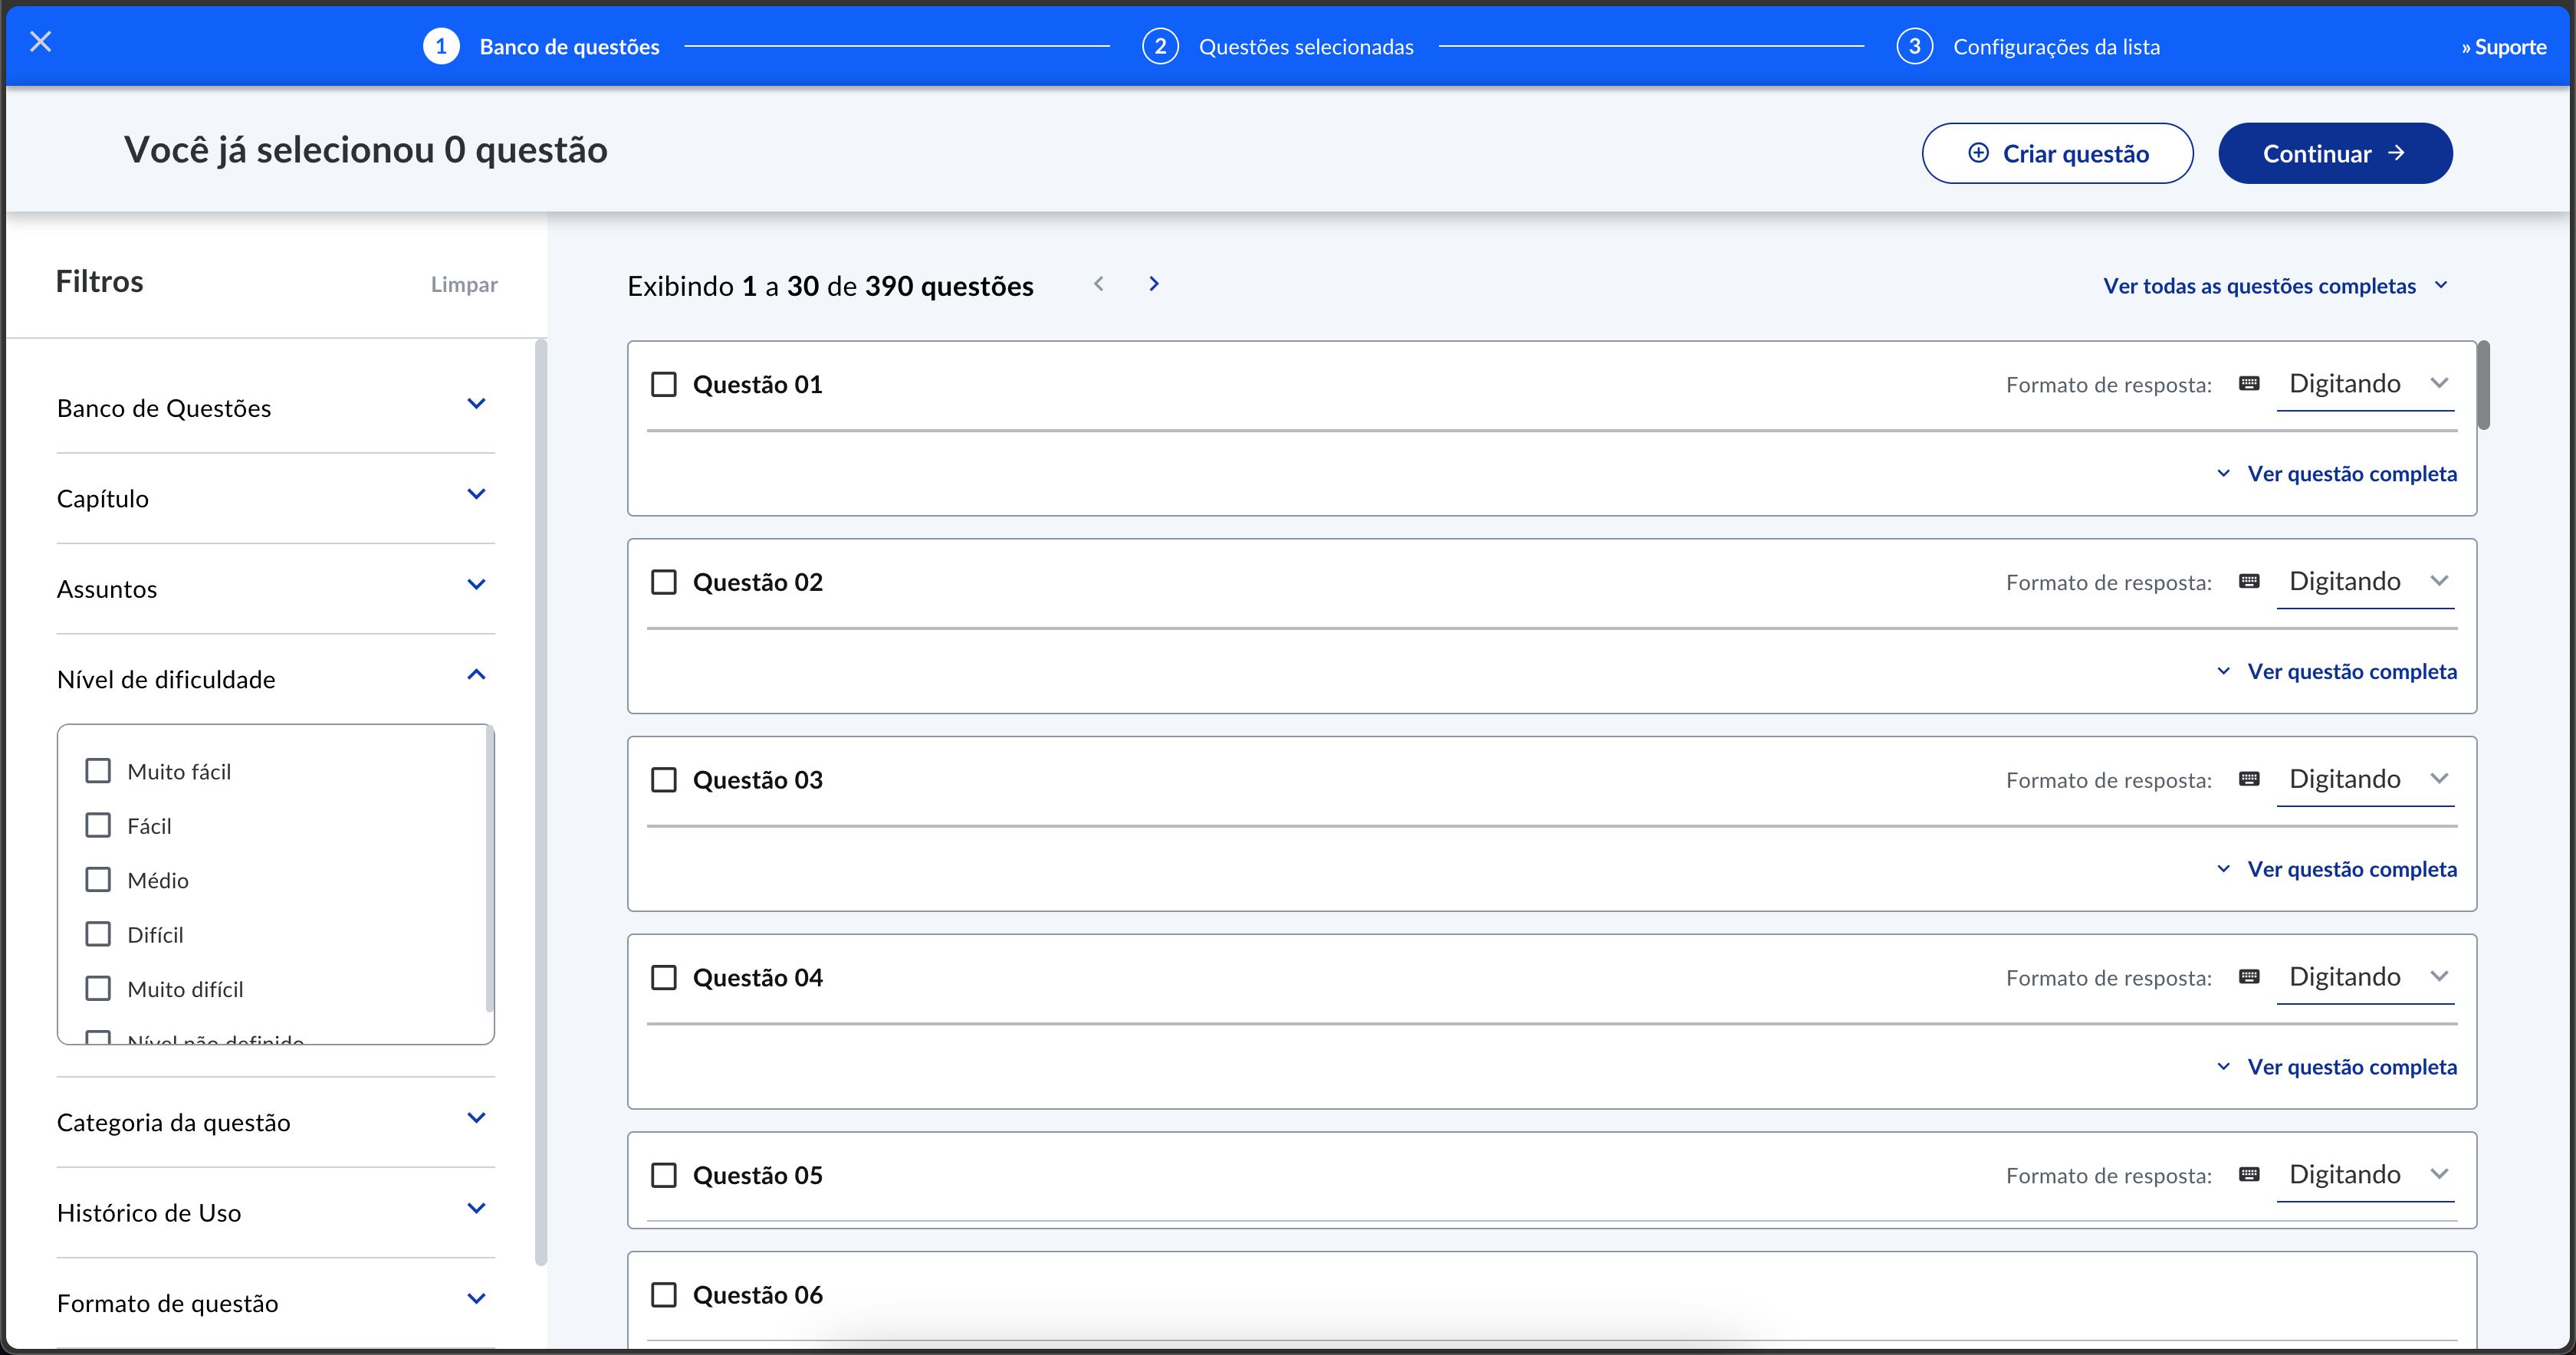
\includegraphics[width=1\linewidth]{figuras/selecao-questoes-tratamento.png}
    \begin{center}
        \text{Fonte: Autor}
    \end{center}
    \label{fig:selecao-questoes-tratamento}
\end{figure}

\begin{table}[]
\centering

    \caption{\textit{Design} do Experimento}

    \begin{tabular}{|c|cl|}
        \hline
        \multirow{2}{*}{População} & \multicolumn{2}{c|}{Fator} \\ \cline{2-3} 
         & \multicolumn{2}{c|}{Posição do Filtro} \\ \hline
        Controle & \multicolumn{2}{c|}{Tratamento A (Última Posição)} \\ \hline
        Tratamento (Usuários Beta) & \multicolumn{2}{c|}{Tratamento B (Quarta Posição)} \\ \hline
    \end{tabular}

    \begin{center}
        \text Fonte: Autor
    \end{center}

    \label{tab:design}
\end{table}

Além disso, foram planejadas medidas para se mitigar possíveis erros nos testes estatísticos. Para mitigar erros do tipo I foi definido um nível de significância alfa de 5\%, a fim de evitar a rejeição da hipótese nula indevidamente (95\% de confiança). Além disso, valores extremos serão removidos do conjunto antes da realização dos testes através de métodos de redução de dados, à depender de qual for mais adequado para a amostra coletada.

Já com relação a erros do tipo II, onde não se rejeita a hipótese nula quando se deveria, foi planejado aumentar o conjunto de dados se possível e se necessário, a fim de aumentar o poder estatístico do teste. Ou seja, o experimento será executado durante um determinado período e, caso as análises se demonstrem inconclusivas por alguma razão, novas iterações serão realizadas. Desta maneira se diminui a probabilidade do erro tipo II sem aumentar a probabilidade de um erro tipo I.

Com todas esta definições previamente realizadas seguiu-se para a instrumentação e pré-estudo do experimento, conforme planejado no processo proposto (ver Subseção \ref{sec:procedimentos}).

\subsection{Instrumentação e Pré-estudo do Experimento}
\label{subsec:pre-estudo}

A instrumentação deste experimento consistiu no preparo da coleta de dados para realização do experimento. Não foi necessária a configuração do Mixpanel \cite{mixpanel2024} nem adição de novos enventos, visto que o produto já teve seu ambiente preparado e já emitia eventos de uso do filtro, de atividades criadas e de exercícios selecionados previamente. Foi necessário apenas a criação de um ambiente de análise e preparação de todo o ferramental, com a criação de um \textit{Jupyter Notebook} \cite{jupyter_notebook} que consumia a API do Mixpanel \cite{mixpanel2024}.

Nesta fase também foi realizado um pré-estudo do experimento. Este procedimento, já apresentado anteriormente, visa verificar se a realização do experimento seria possível nas condições planejadas (população de usuários, métricas selecionadas, etc). Utilizando-se de um teste A/A, que consta em analisar dados de uso onde ambas as populações são apresentadas a mesma versão (de controle), para verificar se o comportamento dos dois grupos de usuários não se comportavam de maneira diferente antes mesmo da implantação da versão de tratamento \cite{SCHERMANN201841}. Este tipo de teste já foi abordado na literatura, e é utilizado para se aumentar a confiabilidade dos experimentos e avaliar o \textit{design} dos mesmos antes de sua execução \cite{fabijan_evolution_2017, fabijan_three_2019, erthal_characterization_2023, fabijan_benefits_2017, crook_seven_2009}.

Foram coletadas então as métricas já definidas no planejamento (número de usos do filtro, de atividades criadas e de exercícios selecionados) além da métrica de interesse da suposição da equipe (proporção de adoção do filtro por nível de dificuldade). Esse procedimento ocorreu entre 08 e 21 de outubro de 2024. Foram registrados 41516 eventos de uso de filtros na seleção de exercícios por 2864 usuários únicos, dos quais 401 pertenciam ao grupo de tratamento (14\%). Os dados foram processados para classificar cada uso do filtro por usuário. Isso possibilitou verificar quantos usuários escolheram a opção de nível de dificuldade pelo menos uma vez. 

Para realizar esta análise, utilizou-se o teste qui-quadrado para comparar os grupos, por se tratar de uma variável categórica: usuário usou ou não o filtro alguma vez no período (uma maior discussão sobre este teste é feita em \ref{subsec:chi-square}). O resultado apontou ausência de diferença significativa (p-valor \(\approx\) 0.94), como mostrado na Figura \ref{fig:pre-study-adocao}. Isso indica que a proporção de adoção do filtro era similar entre os grupos, permitindo a continuidade do experimento.



\begin{figure}[H]
    \centering
    \caption{Teste Sobre Adoção do Filtro de Nível de Dificuldade no Pré-estudo}
    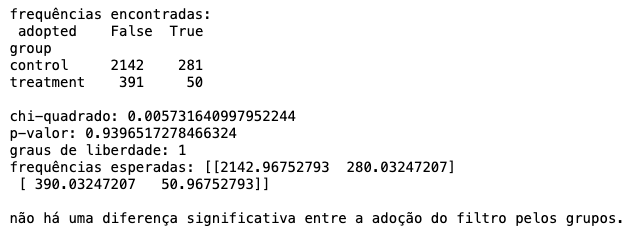
\includegraphics[width=0.85\linewidth]{figuras/pre_study_adocao.png}
    \begin{center}
        \text{Fonte: Autor}
    \end{center}
    \label{fig:pre-study-adocao}
\end{figure}


Em seguida, realizou-se um teste de hipótese sobre a distribuição do número de utilizações do filtro por docente no período. Um teste de hipótese pressupõe que a distribuição dos dois conjuntos é igual, então o resultado visa verificar se há diferença significativa entre os dois grupos. Como os dados não seguiam uma distribuição normal, como pode ser verificado através do histograma apresentado na Figura \ref{fig:pre-study-uses} aplicou-se o teste Mann-Whitney U, que é mais adequado para distribuições não normais (ver Subseção \ref{subsec:u-test}).

Para um nível de significância de 5\%, não foi encontrada diferença estatisticamente significativa na distribuição do número de usos do filtro de nível de dificuldade entre os dois grupos. Os resultados obtidos foram uma estatística \textit{U} de 5511 e um p-valor de 0.7014. 

Uma estatística \textit{U} elevada (mais distante de 0) sugere uma maior similaridade entre as distribuições dos grupos analisados. O p-valor, por sua vez, quantifica a probabilidade de se obter um resultado tão extremo quanto o observado, assumindo que a hipótese nula (de que as duas distribuições são iguais) seja verdadeira. Neste experimento, considerando um limiar de significância de 0.05, um p-valor inferior a esse valor indicaria uma diferença estatisticamente significativa entre os grupos. No entanto, como o p-valor obtido (0.7014) é muito superior a esse limite, conclui-se que não há evidências suficientes para rejeitar a hipótese nula e, portanto, não foi identificada uma diferença estatisticamente relevante entre as distribuições.


% Na figura \ref{fig:pre-study-usos} é ilutratado o comportanmento das distribuições dos grupos de controle (azul) e tratamento (marrom). Foram analisados 331 docentes que utilizaram o filtro pelo menos uma vez (281 no grupo de controle e 50 no de tratamento). O resultado observado evidencia a similaridade do comportamento dessas distribuições. Ou seja, os grupos apresentaram padrões semelhantes em relação ao uso do filtro de nível de dificuldade. Portanto, não houve evidência estatisticamente significativa para concluir que havia associação entre o uso do filtro e os diferentes tratamentos.
 
\begin{figure}
    \centering
    \caption{Distribuições do Número de Utilizações do Filtro no Pré-estudo}
    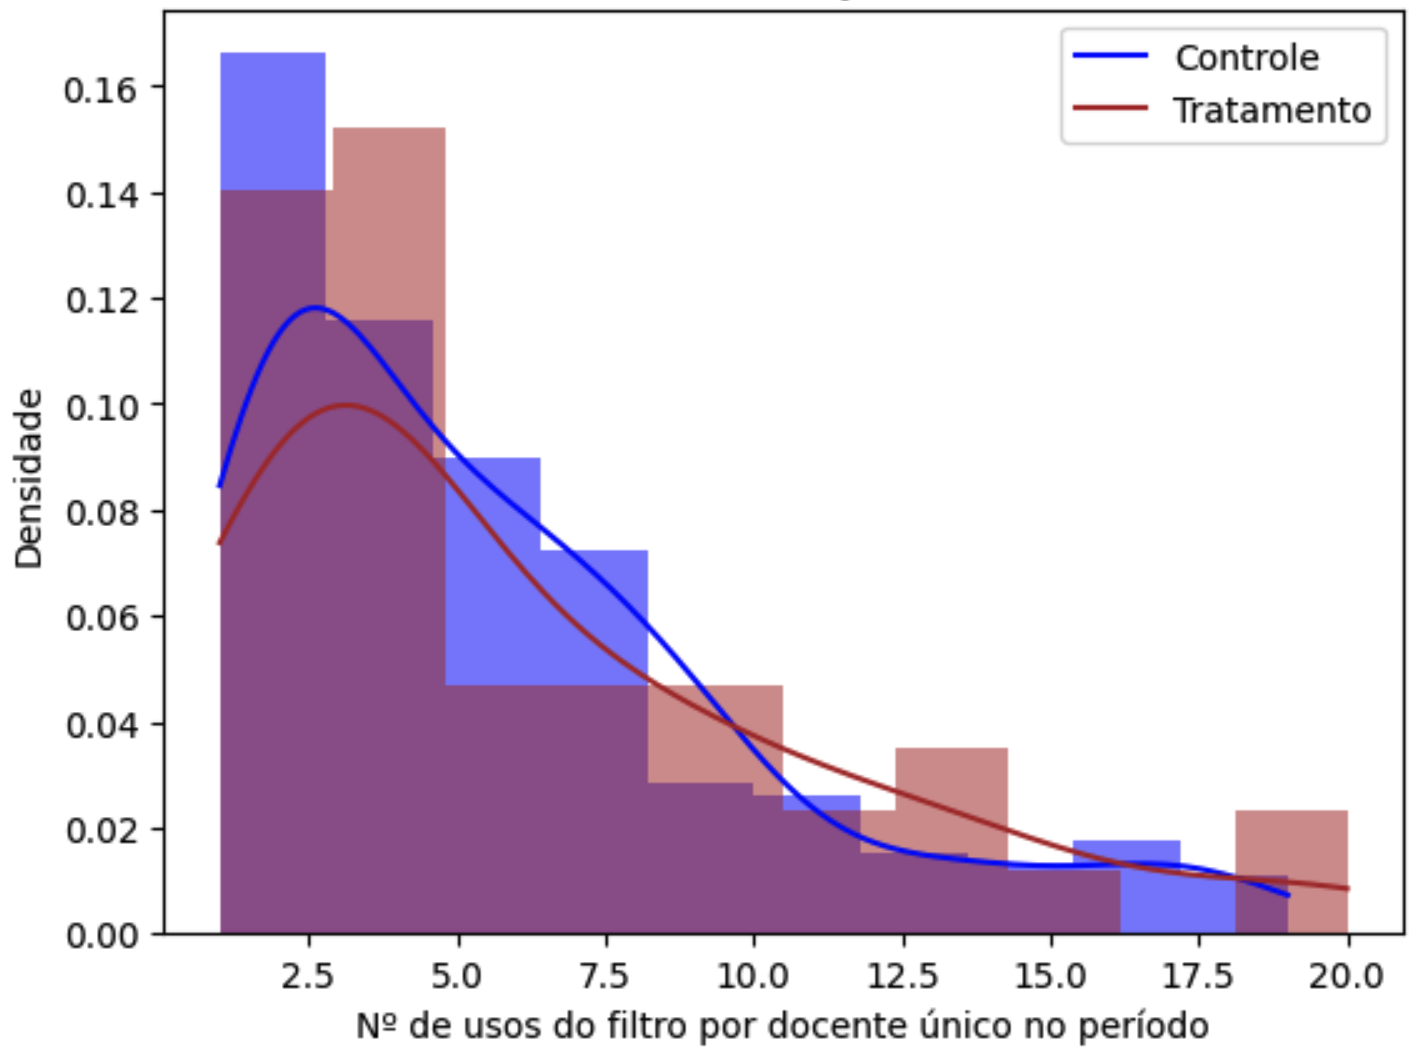
\includegraphics[width=0.85\linewidth]{figuras/pre-study-usos.png}
    \begin{center}
        \text{Fonte: Autor}
    \end{center}
    \label{fig:pre-study-usos}
\end{figure}

Ainda no intuito de testar os procedimentos a serem utilizados na execução do experimento planejado... blá, blá, blá...

Ainda no intuito de se testar a similaridade do comportamento dos dois grupos, outro teste foi conduzido para avaliar a distribuição do número de listas de exercícios criadas por docente (outra das varíaveis escolhidas para análise). Novamente, utilizou-se o teste Mann-Whitney U, dada a ausência de normalidade nos dados (como pode ser verificado no histograma apresentado na Figura \ref{fig:pre-study-acts}). Para um nível de significância de 5\%, não houve diferença significativa entre os grupos (\textit{U} = 4797, p = 0.3166). No total, foram considerados 269 docentes que criaram ao menos uma atividade e utilizaram o filtro (224 no grupo de controle e 45 no de tratamento).

\begin{figure}
    \centering
    \caption{Distribuições do Número de Listas de Exercícios Criadas no Pré-estudo}
    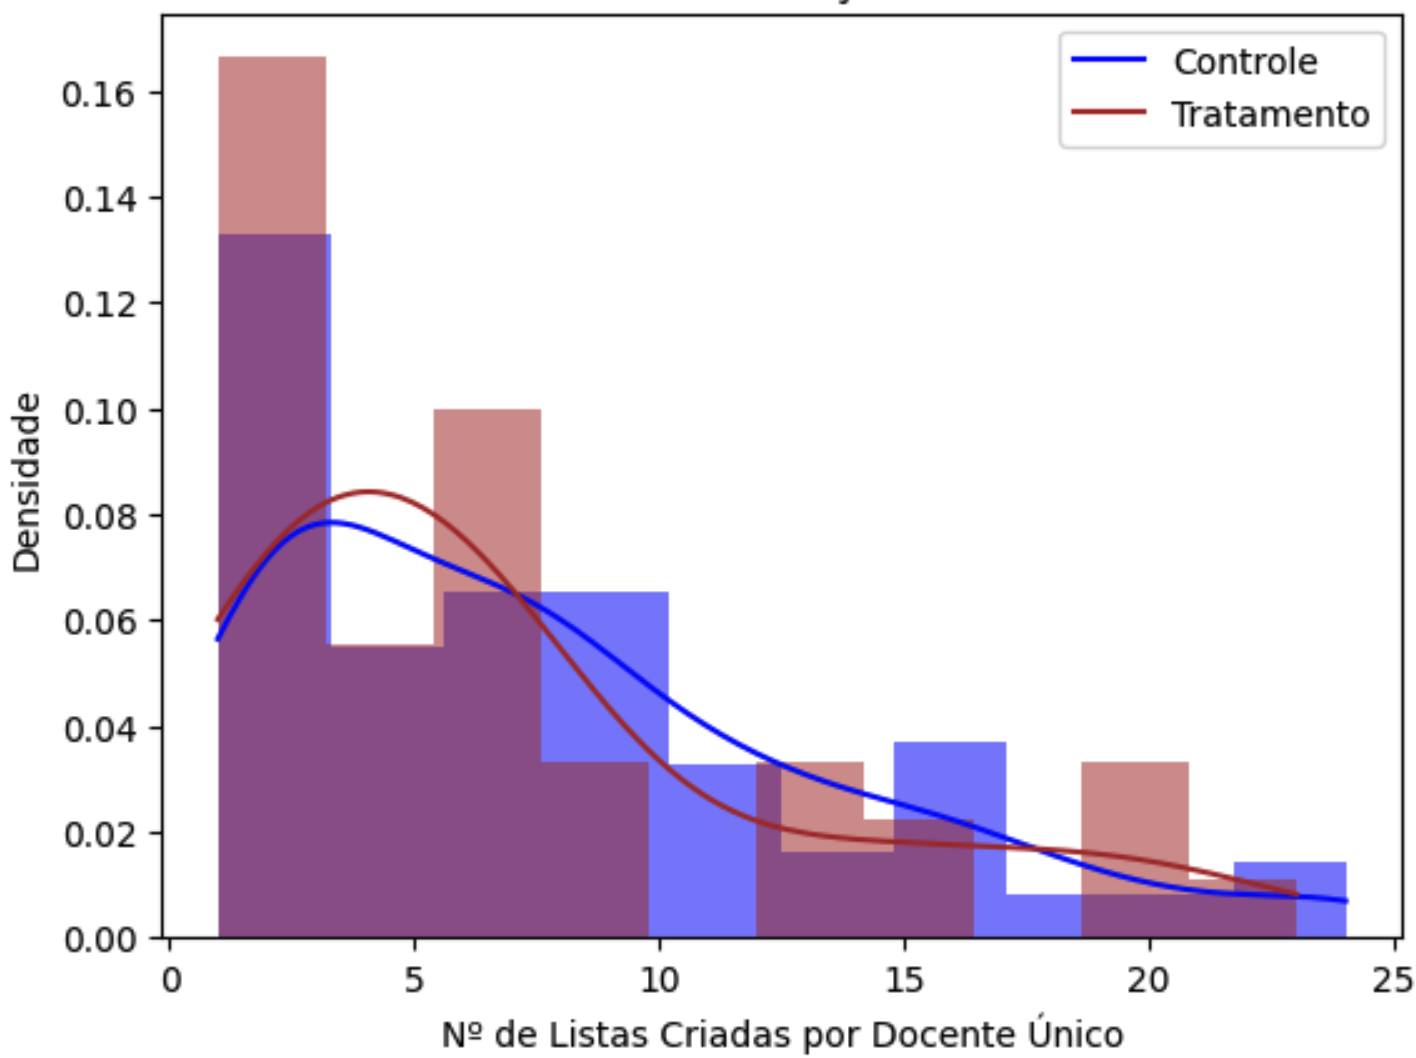
\includegraphics[width=0.85\linewidth]{figuras/pre-study-acts.png}
    \begin{center}
        \text{Fonte: Autor}
    \end{center}
    \label{fig:pre-study-acts}
\end{figure}

Por fim, para se finalizar este pré-estudo, testou-se a distribuição do número de exercícios selecionados por docente no período. Utilizou-se novamente o teste Mann-Whitney U (distribuições distribuições são apresentadas na Figura \ref{fig:pre-study-exs}). Para um nível de significância de 5\%, não foi observada diferença significativa entre os grupos (\textit{U} = 4780.5, p = 0.4772). No total, 269 docentes foram analisados (224 do grupo de controle e 45 do grupo de tratamento).


\begin{figure}
    \centering
    \caption{Distribuições do Número de Exercícios Selecionados no Pré-estudo}
    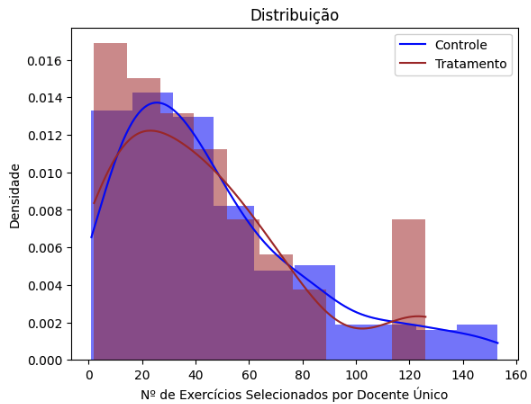
\includegraphics[width=0.85\linewidth]{figuras/pre-study-exs.png}
    \begin{center}
        \text{Fonte: Autor}
    \end{center}
    \label{fig:pre-study-exs}
\end{figure}

Após essas análises\footnote{Os dados coletados foram anonimizados e disponibilizados em repositório público, junto com os cadernos de análise. Disponível em: \href{https://github.com/senaarth/tcc-notebooks/blob/main/pre-study.ipynb}{https://github.com/senaarth/tcc-notebooks}}, concluiu-se que não havia diferenças no comportamento dos grupos antes da introdução da nova versão. Esse processo foi realizado a partir de considerações encontradas na literatura estudada e visou aumentar a confiabilidade das análises subsequentes (uma maior discussão é realizada na Subseção \ref{subsec:relacionados}) \cite{fabijan_evolution_2017, fabijan_three_2019, erthal_characterization_2023, fabijan_benefits_2017, crook_seven_2009}. Assim, prossegui-se com a execução do experimento planejado na Subseção anterior, \ref{subsec:plan_exp}.
